\def\auth{Carlos Salinas}
\def\tight{MRC 2016 Report: Tropicalization of Character Varieties}
\def\short{Trop-Summ}
\def\class{tropicalization}
\def\subject{character varieties, tropical geometry, tropicalization}
\def\eemail{salinac@purdue.edu}

\documentclass[11pt]{article}

\usepackage[dvipsnames]{xcolor}%
\usepackage{geometry}
\usepackage[%
breaklinks,%
colorlinks=true,%
linkcolor=black,%
citecolor=black,%
filecolor=black,%
menucolor=black,%
runcolor=black,%
urlcolor=black,%
pdftitle={\short},%
pdfauthor={\auth},%
pdfkeywords={\subject},%
pdfsubject={\class},%
pageanchor={false}%
]{hyperref}

% TOC depth
%% Math and variables all bundled up
\usepackage{carlos-variables}

%% Misc
\usepackage{microtype}
\usepackage[inline]{enumitem}
\usepackage{graphicx}
\graphicspath{{figures/}}
\usepackage{authblk}
\DeclareMathOperator{\Newt}{Newt}

\begin{document}

%% Footnote style
\renewcommand*{\thefootnote}{\fnsymbol{footnote}}

%% Title

\author[1]{Shams Alyusof}
\author[4]{Corry Bedwell}
\author[2]{Ellie Dannenberg}
\author[5]{Dmitry Gekhtman}
\author[1]{Charlie Katerba}
\author[1]{Jack Love}
\author[1]{Christopher Manon}
\author[3]{Giuseppe Martone}
\author[6]{\href{mailto:\eemail}{\auth}}%
\affil[1]{George Mason University}
\affil[2]{University of Illinois at Chicago}
\affil[3]{University of Southern California}
\affil[4]{University of Maryland--College Park}
\affil[5]{California Institute of Technology}
\affil[6]{Purdue University}

\renewcommand\Authands{ and }
\title{\tight}%
% \author{\auth}
\date{\today}%

\maketitle
% \tableofcontents
\section{Overview}
Tropical geometry is a new an exciting area of mathematics that is best
described as a piecewise-linear version of algebraic geometry. In tropical
geometry the sum of two real numbers $x\oplus y$ is their maximum and the
product $x\odot y$ their sum. This, together with a minimum element
$-\infty$, gives us the tropical semiring
$(\bbR\cup\{-\infty\},\oplus,\odot)$. In the tropical setting, polynomials
become pice-wise linear functions and algebraic varieties give way to
tropical varieties--- which are in some sense ``skeletons'' of the original
variety.

During the introductory talks by Manon, we decided to try our hand at
\emph{tropicalizing} some of the $\SL(2,\bbC)$-character varieties that
were presented Lawton's talk and, further, tropicalize $\PSL(2,\bbC)$-,
$\SL(3,\bbC)$-, an $\Sp(4)$-character varieties. We broke
out---loosely---into two groups: one concerned with the tropicalization of
$\PSL(2,\bbC)$-character varieties and the other with visualization of the
Newton polytopes that came about from tropicalization.

Here is a summary of the observations made by the group.

\section{Tropicalization of $\frakX(F_3,\SL(2,\bbC))$}
From Lawton \cite{0601132} Corollary 4 and Lemma 5, and some
\texttt{Mathematica} Gröbner basis magic, we deduced that the coordinate
ring of the character variety $\frakX(F_3,\SL(2,\bbC))$ is cut out by the
polynomial in $7$ indeterminates
\begin{equation}
  \label{eq:f3-sl2c}
  \begin{aligned}
    f=X_1X_2X_3X_7&-{X_4}^2+{X_5}^2+{X_1}^2\\
    &+{X_2}^2+{X_3}^2+{X_7}^2\\
    &+X_1X_6X_7+X_2X_5X_7+X_3X_4X_7\\
    &+X_1X_2X_4+X_1X_3X_5+X_2X_3X_6-4.
  \end{aligned}
\end{equation}

With the help of \texttt{gfan}---a software package for computing Gröbner
fans and tropical varieties \cite{gfan}---and \texttt{Mathematica} we were
were able to find $\Trop(\frakX(F_3,\SL(2,\bbC)))$. Its tropicalization is
the codimension $1$-cones of the dual fan to the Newton polytope
$\Newt(f)$. Figure \ref{fig:f3-sl2c} is a picture made we made using the
Ti\textit{k}Z graphics language to draw the edge graph of $\Newt(f)$

\begin{figure}[htpb]
  \centering
  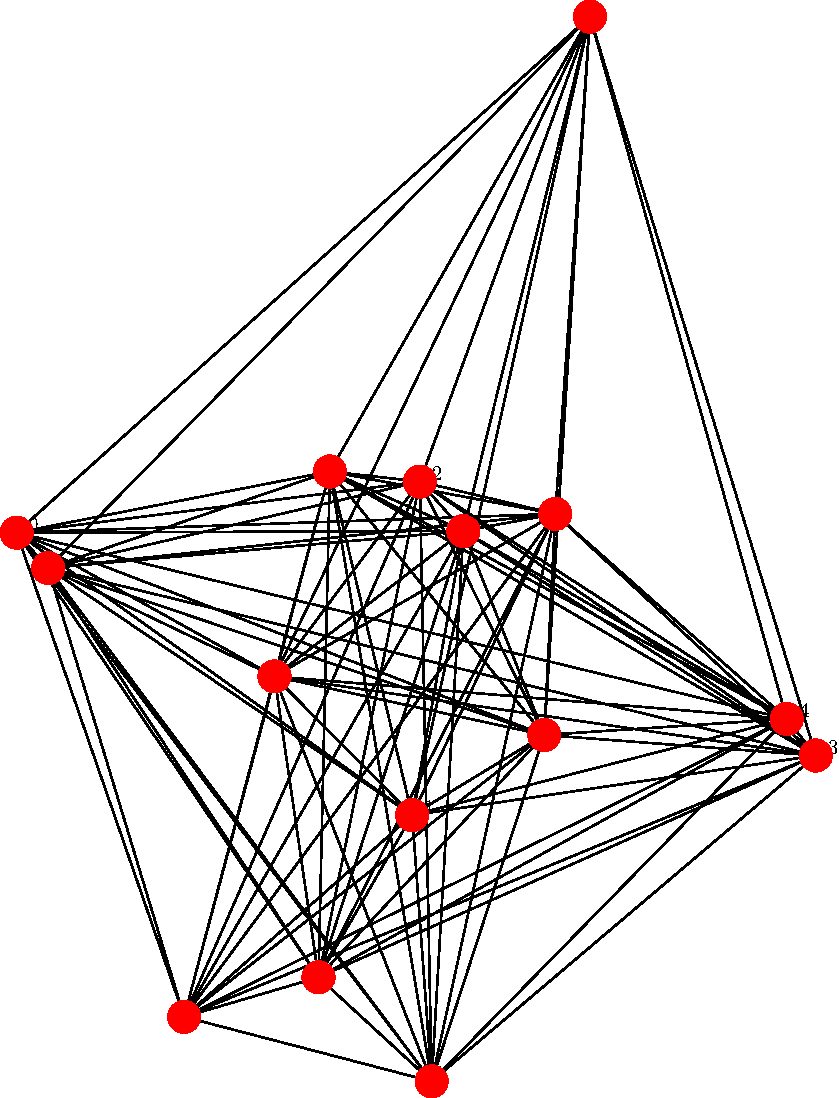
\includegraphics[scale=.25]{smallgraph}
  \caption{Edge graph of the Newton polytope of $\frakX(F_3,\SL(2,\bbC))$.}
\label{fig:f3-sl2c}
\end{figure}

More information about its tropicalization was extracted using
\texttt{gfan}. The relevant file is on the MRC website under the
\texttt{Tropical Group Files/F\_3->SL\_2} folder with the tile
\texttt{hypersurface\_F3->SL(2,C)\_groebnerfan.txt}.

\section{Tropicalization of  $\frakX(F_2, \SL_3\bbC))$}
The coordinate ring of the character variety $\frakX(F_2, \SL_3\bbC))$ is
cut out by the huge polynomial in $9$ indeterminates
\begin{equation}
  \label{eq:f2-sl3c}
  \begin{aligned}
    f=9&+3X_9 - 6X_1X_2\\
    &-6X_3X_4-6X_5X_6-6X_7X_8 + {X_9}^2- X_1X_2X_9\\
    & - X_3X_4X_9 - X_5X_6X_9\ - X_7X_8X_9+{X_1}^3\\
    &+ {X_3}^3 + {X_5}^3 + {X_7}^3 + {X_2}^3 \\
    &+ {X_4}^3 + {X_6}^3 + {X_8}^3 - 3X_2X_8X_6\\
    &- 3X_1X_5X_7 - 3X_3X_5X_8-3X_4X_6X_7 + 3X_1X_4X_8\\
    &+ 3X_2X_3X_7 + 3X_1X_3X_6 + 3X_2X_4X_5 - X_1X_2X_3X_4X_9\\
    &+ X_1X_3X_6X_9 + X_2X_4X_5X_9 + X_1X_4X_8X_9+X_2X_3X_7X_9\\
    &+ X_1X_2X_3X_4 + X_3X_4X_5X_6+ X_1X_2X_7X_8 + X_3X_4X_7X_8\\
    &+ X_1X_2X_5X_6+ X_5X_6X_7X_8 + X_4{X_8}^2X_6 + X_3X_5{X_7}^2\\
    &+ {X_2}^2X_4X_8 + {X_1}^2X_3X_7 + X_1{X_4}^2X_6 + X_2{X_3}^2X_5\\
    &+ {X_1}^2X_8X_6 + {X_2}^2X_5X_7+ X_3X_8{X_6}^2 + X_4{X_5}^2X_7 \\
    &+ {X_2}^2X_3X_6 + {X_1}^2X_5X_4 + X_1{X_3}^2X_8 + X_2{X_4}^2X_7\\
    &+ {X_4}^2X_5X_8 + {X_3}^2X_6X_7+ X_1X_5{X_8}^2 + X_2X_6{X_7}^2 \\
    &+ X_2{X_5}^2X_8 + X_1{X_6}^2X_7 - 2X_2X_4{X_6}^2 - 2X_1X_3{X_5}^2\\
    &- 2X_2X_3{X_8}^2 - 2X_1X_4{X_7}^2+ {X_2}^2{X_4}^2X_6 +
    {X_1}^2{X_3}^2X_5\\
    &+ {X_2}^2{X_3}^2X_8 + {X_1}^2{X_4}^2X_7- X_1X_3{X_4}^2X_8 -
    X_2{X_3}^2X_4X_7\\
    &- {X_1}^2X_2X_3X_6 - X_1{X_2}^2X_4X_5- X_1{X_3}^2X_4X_6 -
    X_2X_3{X_4}^2X_5\\
    &- {X_1}^2X_2X_4X_8- X_1{X_2}^2X_3X_7 - X_1X_2{X_4}^3 - X_1X_2{X_3}^3\\
    &- {X_2}^3X_3X_4 - {X_1}^3X_3X_4- X_2X_3X_4X_8X_6 - X_1X_3X_4X_5X_7\\
    & - X_1X_2X_3X_5X_8- X_1X_2X_4X_6X_7 + {X_1}^2{X_2}^2X_3X_4 +
    X_1X_2{X_3}^2{X_4}^2
  \end{aligned}
\end{equation}
The edge graph of its Newton polytope is shown in Figure \ref{fig:f3-sl3c}.

\begin{figure}[htpb]
  \centering
  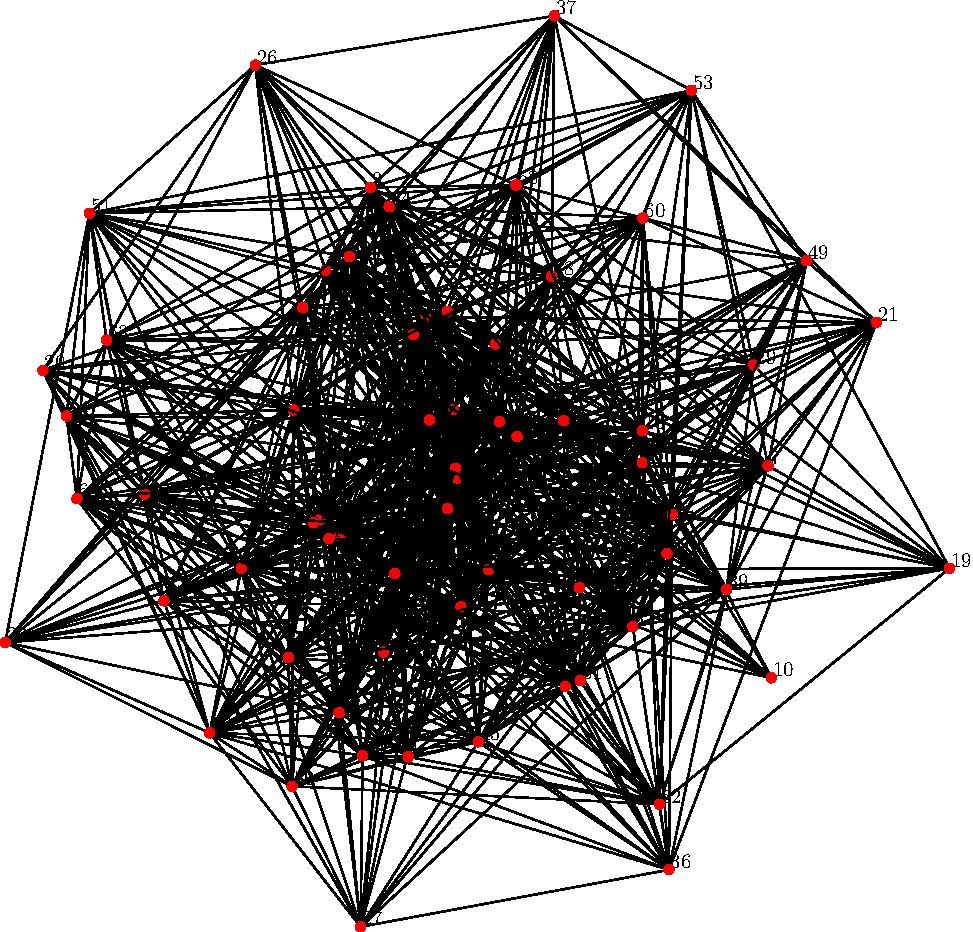
\includegraphics[scale=.55]{biggraph}
  \caption{Edge graph of the Newton polytope of
    $\frakX(F_3,\SL(3,\bbC))$.}
\label{fig:f3-sl3c}
\end{figure}

More information about the tropicalization of was extracted using
\texttt{gfan}. The file containing this information (is huge) can be found
on the MRC website under the \texttt{Tropical Group Files/F\_2->SL\_3}
folder with title \texttt{F\_2SL\_3TropicalVariety}. \textbf{Warning} the
file is huge.

\section{Tropicalization of $\PSL(2,\bbC)$-character varieties}
In addition to tropicalizing plain $\SL(2,\bbC)$- and
$\SL(3,\bbC)$-character varieties, we decided to look at $\PSL(2,\bbC)$-
and $\Sp(4)$-character varieties.

Let $F_3$ be the free group on $3$ generators $A,B,C$. Then, we claim that
the coordinate ring of $\frakX(F_3,\PSL(2,\bbC))$
\[
  \bbC[\frakX(F_3,\PSL(2,\bbC)]=\bbC[\frakX(F_3,\SL(2,\bbC))]^{\bbZ/2\bbZ\times\bbZ/2\bbZ\times\bbZ/2\bbZ}
\]
is cut out the following family of trace-polynomials---which we shall group
according to similarity:
\begin{itemize}
\item Type $\chi$:
  \begin{align*}
    \chi_A&=(\tr A)^2&\chi_B&=(\tr B)^2&\chi_C&=(\tr C)^2\\
    \chi_{AB}&=(\tr AB)^2&\chi_{AC}&=(\tr AC)^2 \\
    \chi_{BC}&=(\tr BC)^2&\chi_{ABC}&=(\tr ABC)^2
  \end{align*}
\item Type $\tau$:
  \begin{align*}
    \tau_{AB}&=\tr A\tr B\tr AB &\tau_{AC}&=\tr A\tr C\tr AC &\tau_{BC}&=\tr B\tr C\tr BC
  \end{align*}
\item Type $\Lambda$:
  \begin{align*}
    \Lambda_A&=\tr B\tr C\tr AB\tr AC
    &\Lambda_B&=\tr A\tr C\tr AB\tr BC\\
    \Lambda_C&=\tr A\tr B\tr AC\tr BC
  \end{align*}
\item Lonely $\Delta$:
  \[
    \Delta= \tr A\tr B\tr C\tr ABC
  \]
\item Equally lonely $\Sigma$:
  \[
    \Sigma= \tr AB\tr AC\tr BC
  \]
\item Type $\Theta$:
  \begin{align*}
    \Theta_A&=\tr A\tr BC\tr ABC&\Theta_B&=\tr B\tr AC\tr ABC \\
    \Theta_C&=\tr C\tr AB\tr ABC
  \end{align*}
\end{itemize}

With some further algebraic manipulations, we observe the following
relations among the generators
\[
  \Sigma ^2=(\tr AB\tr AC\tr BC)^2=\chi_{AB}\chi_{AC}\chi_{BC}
\]
and some binomial relations
\begin{align*}
  \tau_{AB}^2&=\chi_A\chi_B\chi_{AB} &\tau_{AC}^2&=\chi_A\chi_C\chi_{AC}\\
  \tau_{BC}^2&=\chi_B\chi_C\chi_{BC}\\\\
  \Lambda_A^2&=\chi_B\chi_C\chi_{AB}\chi_{AC}
  &\Lambda_B^2&=\chi_A\chi_C\chi_{AB}\chi_{BC}\\
  \Lambda_C^2&=\chi_A\chi_B\chi_{AC}\chi_{BC}\\\\
  \Theta_A^2&=\chi_A\chi_{BC}\chi_{ABC}&\Theta_B^2&=\chi_B\chi_{AC}\chi_{ABC}\\
  \Theta_C^2&=\chi_C\chi_{AB}\chi_{ABC}\\\\
  \Sigma ^2&=\chi_{AB}\chi_{AC}\chi_{BC}&\Delta^2&=\chi_A\chi_B\chi_C\chi_{ABC}.
\end{align*}
and finally the relation coming from $\frakX(F_3,\SL(2,\bbC))$
\begin{align*}
  \chi_A+\chi_B+\chi_C+\chi_{AB}+\chi_{AC}
  &=\tau_{AB}+\tau_{AC}+\tau_{BC}\\
  +\chi_{BC}+\chi_{ABC}+\Sigma+\Delta
  &\phantom{{}={}}+\Theta_A+\Theta_B+\Theta_C+4.
\end{align*}

On the last day of the MRC we further managed to tropicalize
$\frakX(F_2,\Sp(4))$. The Gröbner basis and other tropicalization
information we obtained from \texttt{gfan} can be found on the MRC website
under the \texttt{Tropical Group Files/F\_2->SP\_4}.

\section{Visualization of character varieties of knot complements}
Although \texttt{gfan} can make excellent polyhedral representation of the
Gröbner fans we obtained from the tropicalization of our character
varieties, the documentation is very sparse and so we tried our hand at
making these polyhedral representations from scratch using
\texttt{Mathematica} which, surprisingly enough, does not yet have great
support for tropical geometry.

We attempted to create the Newton polytopes of several knot groups whose
$A$-polynomials we obtained from a paper by Eric Chesebro \emph{Formulas
  for Character Varieties of $2$-Bridge Knots} which can be found on the
University of Montana's Department of Mathematical Sciences, Technical
reports page under the Research tab. Here is a link to the document in
question
\url{http://hs.umt.edu/math/research/technical-reports/documents/2012/KnotFormulas.pdf}.

With the help of \texttt{Mathematica}, we made the following subdivision of
the Newton polytopes of these character varieties.
\begin{figure}[htpb]
  \centering
  
\includegraphics[scale=0.5]{newtonsub_apoly_fig8}
  \caption{Subdivided Newton polytope for the $A$-polynomial of the
    figure-$8$ knot.}
  \end{figure}

\begin{figure}[htpb]
  \centering
  
\includegraphics[scale=0.45]{newtonsub_apoly_twist4}
  \caption{Subdivided Newton polytope for the $A$-polynomial the
    $4$-twisted knot.}
\end{figure}

Some more pictures for Newton polytopes of two $2$-bridge knots
corresponding to $\varphi(1)$ and $\varphi(2)$ of Chesebro's equation are
shown in Figures \ref{fig:phi1} and \ref{fig:phi2}.
\begin{figure}[htpb]
  \centering
  
\includegraphics[scale=0.5]{newtonsub_phi1}
  \caption{Subdivided Newton polytope for the $A$-polynomial of the
    $\varphi(1)$ $2$-bridge knot.}
  \label{fig:phi1}
\end{figure}
\begin{figure}[htpb]
  \centering
  
\includegraphics[scale=0.5]{newtonsub_phi2}
  \caption{Subdivided Newton polytope for the $A$-polynomial of the
    $\varphi(1)$ $2$-bridge knot.}
  \label{fig:phi2}
\end{figure}

The dual of these images is really what we are after and, although we may
be on hiatus for the moment, we plan to finish writing the code that does
this.

\newpage
\bibliographystyle{acm}
\bibliography{trop-charvar}
\end{document}

%%% Local Variables:
%%% mode: latex
%%% TeX-master: t
%%% End:
